% E0240 Project 1, Phase-1 problem statement (due 22 September 2026).
% NOTE: the "Group members" line in the title block is a placeholder:
% fill in teammate names and SR numbers, or delete the line, before submission.
% Real-system numbers in Table 1 are flagged "representative" on purpose:
% swap in measured values if you want them attributed to your own benchmarking.
\documentclass[11pt,a4paper]{article}
\usepackage[utf8]{inputenc}
\usepackage[margin=1.5cm,footskip=25pt]{geometry}
\usepackage{amsmath,amssymb}
\usepackage{microtype}
\usepackage{booktabs}
\usepackage{float}
\usepackage{caption}
\captionsetup{font=small,labelfont=bf,skip=4pt}
\usepackage{tikz}
\usetikzlibrary{arrows.meta,positioning,calc}
\usepackage[hidelinks]{hyperref}

\setlength{\parskip}{1.5pt}
\emergencystretch=1em
\makeatletter
\renewcommand\section{\@startsection{section}{1}{\z@}%
  {-3.1ex plus -0.6ex minus -.2ex}{1.6ex plus .2ex}{\normalfont\Large\bfseries}}
\makeatother
\setlength{\intextsep}{4pt plus 1pt minus 1pt}

\title{\vspace{-2.2em}\textbf{\huge E0240: Modeling and Simulation}\\[0.4em]
\Large \textbf{Project Phase-1: Problem Statement}\\[0.3em]
\large A Queueing-Network Simulator for an LLM Inference Serving Pipeline}
\author{\textbf{Name:} Vaibhav Mahore \quad \textbf{SR No.:} 23631\\[0.2em]
\textit{UG BTech (M\&C)}, Department of Computer Science and Automation (CSA)\\[0.2em]
\textbf{Indian Institute of Science, Bangalore}\\[0.2em]
\textbf{Group members:} \textit{[Name (SR No.)] \quad [Name (SR No.)]}}
\date{\textbf{Submission Date:} 22 September 2026}

\begin{document}
\maketitle
\vspace{-0.4em}
\hrule
\vspace{1.2em}

\section*{1. Why an LLM Inference Serving Pipeline}
Large language model (LLM) inference serving is a real-time system. A user watches
tokens appear one by one, so both the wait for the first token and the speed after
it are directly visible, and serving systems carry strict latency targets on
exactly these quantities. Behind the API, the serving stack (engines such as vLLM)
is essentially a chain of queues. A request is admitted and tokenized, then held by
a scheduler until a batch is ready, and finally decoded on GPU workers, where the
service time depends on how many tokens the answer turns out to need. At each of
these stages the user-visible latency is mostly waiting: requests waiting in the
admission queue, waiting for a batch to fill, or waiting for a free worker. Queue
occupancy therefore connects directly to what the user feels, which is why we made
it the key performance metric of the simulator.

Batching is what makes the system worth modeling. A larger batch gives better
throughput and GPU utilization, but every request in it waits longer for the batch
to fill. This waiting-versus-throughput trade-off is the kind of question a
queueing network handles naturally, and the scheduler settings (batch size, wait
timer, number of workers) are the knobs we plan to sweep.

There is also a practical reason to simulate: real serving clusters are shared and
expensive, so sweeping injection rate, batch size and worker count in a small
discrete-time model is far easier than experimenting on a live system, and it shows
the stable and saturated regimes next to each other.

\section*{2. The Queueing Network Abstraction}
We model the pipeline as an open queueing network of three stations connected in a
single path, in the same spirit as a road traffic network drawn as a network of
queues, where each station carries its own arrival and service rate. Figure 1
shows the stations. Requests pass through each station once, so in steady state all
three see the same injection rate $\lambda$ (requests per cycle, with requests
playing the role of packets). Arrivals are Bernoulli: in each cycle a request
arrives with probability $\lambda$.

\begin{figure}[H]
\centering
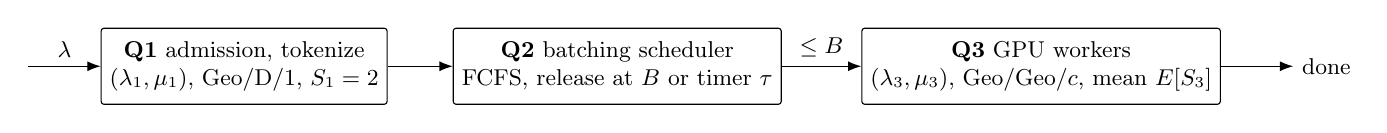
\begin{tikzpicture}[>=Latex, font=\small, scale=0.92, transform shape,
  stn/.style={draw, rounded corners=1pt, minimum width=3.1cm, minimum height=1.05cm, align=center}]
\node[stn] (q1) {\textbf{Q1} admission, tokenize\\ $(\lambda_1,\mu_1)$, Geo/D/1, $S_1=2$};
\node[stn,right=0.9cm of q1] (q2) {\textbf{Q2} batching scheduler\\ FCFS, release at $B$ or timer $\tau$};
\node[stn,right=1.1cm of q2] (q3) {\textbf{Q3} GPU workers\\ $(\lambda_3,\mu_3)$, Geo/Geo/$c$, mean $E[S_3]$};
\draw[->] ($(q1.west)+(-1.0,0)$) -- node[above]{$\lambda$} (q1.west);
\draw[->] (q1) -- (q2);
\draw[->] (q2) -- node[above]{$\le B$} (q3);
\draw[->] (q3.east) -- ++(1.0,0) node[right]{done};
\end{tikzpicture}
\caption{The LLM serving pipeline as a three-station queueing network.}
\end{figure}

\textbf{Q1, admission and tokenization.} One server with deterministic service time
$S_1 = 2$ cycles (request parsing, template and budget checks), service law Geo/D/1
with $\mu_1 = 1/S_1$. Setting $S_1 = 2$ was deliberate: the station is then exactly
the standard Geo/D/1 queue, so its analytical results carry over unchanged.

\textbf{Q2, batching scheduler.} A first-come-first-served buffer that releases
requests as one batch when either $B$ requests have collected or the oldest request
has waited $\tau$ cycles, whichever happens first. When $B = 1$ the station is a
plain pass-through, and that is the configuration we use for validation. We model
static batching only, where a batch is closed and dispatched as a group; continuous
batching, where new requests join a running batch, is left as an extension.

\textbf{Q3, GPU workers.} $c$ identical parallel workers (concurrent decoding
slots), first-come-first-served, each serving one request with a geometric service
time of mean $E[S_3]$ cycles, service law Geo/Geo/$c$. Decode length is where most
of the service variability in serving comes from, and geometric service is the
natural discrete-time model for variable job length: a request completes each cycle
with probability $p_s = \mu_3 = 1/E[S_3]$, independently of how long it has already
run. Heavier-tailed service laws are left as a possible extension.

\textbf{Simplifying assumptions.} Each request makes one pass, with no feedback or
routing splits; batching changes only how long requests wait, not how much service
they need; there is no preemption; the workers are identical; arrivals are
Bernoulli as above.

Node $i$ is stable when $\rho_i = \lambda_i E[S_i] < 1$. The path is single and
requests are conserved, so $\lambda_i = \lambda$ at every station, and the
conditions that actually bind are $2\lambda < 1$ at Q1 and $\lambda E[S_3]/c < 1$
at Q3. Q2 only holds requests between the two and is stable as long as Q3 is.
Table 1 collects representative parameter values and maps them to model cycles,
where one model cycle corresponds to one scheduler tick.

\begin{table}[H]
\centering\footnotesize
\caption{Representative parameters mapped to model cycles.}
\begin{tabular}{@{}p{2.5cm}p{4.5cm}p{4.9cm}p{4.3cm}@{}}
\toprule
Quantity & Real system (representative) & Model value & Provenance \\
\midrule
Scheduler tick & 10--50 ms per scheduling pass & one cycle & representative; to be pinned against measured configurations in Phase-2 \\
Arrivals & request stream at the serving endpoint & Bernoulli, prob.\ $\lambda$ per cycle; sweep $[0.05{:}0.05{:}0.45,\,0.49]$ & standard validation sweep \\
Batch capacity $B$ & 8--32 requests per batch & $B \in \{1,4,8,16,32\}$; $B=1$ for validation & representative \\
Batch wait timer $\tau$ & a few scheduler ticks & $\tau \in \{1,2,5,10\}$ cycles & representative \\
Decode length & varies per request, tens of tokens & geometric, mean $E[S_3]=20$ cycles (swept) & geometric law; mean representative \\
Tokenizer service & small, fixed overhead & $S_1 = 2$ cycles, deterministic & standard validation value \\
Decode slots $c$ & 8--32 concurrent sequences per GPU & $c=1$ for validation; 8--32 in experiments & representative \\
\bottomrule
\end{tabular}
\end{table}

\section*{3. Key Performance Metric and Method}
The metrics are the standard discrete-time queueing metrics. At each node we will
track the time-average queue occupancy $L_{q,i} = (1/T)\sum_t Q_i(t)$, computed as
the occupancy counter divided by the simulation length; the average delay per
request $(\sum D_i)/n$ over the $n$ requests completed at that node; and the server
utilization, counted as busy cycles over total cycles. As checks, the measured
utilization should match $\rho_i = \lambda_i E[S_i]$ ($\lambda E[S_3]/c$ at Q3),
and the per-node waiting time $W = L_q/\lambda$ should agree with the directly
measured delays. A request's end-to-end delay is the sum of its delays at the
three nodes.

The simulator will be cycle-driven discrete-time: time advances in fixed increments
of one cycle. In each cycle it (i) draws a uniform random number $U \in [0,1)$ and
admits a request if $U \le \lambda$, (ii) reduces the remaining service time of
busy servers, (iii) sends the head-of-line request, or a released batch, to idle
workers, and (iv) adds to the occupancy and utilization counters before moving on.
Random variates are generated with the inverse transform technique: Bernoulli
arrivals straight from $U \le \lambda$, geometric service from the per-cycle test
$U < p_s$. We will write the simulator in Python and plot with matplotlib, and fix
the random seed so that every run is reproducible.

\section*{4. Validation Plan}
Validation will only use closed-form analytical targets. With Q2 as pass-through
($B=1$) and $c=1$, the network reduces to a single station, and we check two
things. First, with deterministic service $S=2$, the simulated occupancy should
match Geo/D/1, $L_q = \lambda^2 (S-1)/(1-\lambda S) = \lambda^2/(1-2\lambda)$, and
the waiting time should match $W_q = \rho(S-1)/(2(1-\rho))$. Second, with
geometric service of mean $E[S_3]=2$, it should match Geo/Geo/1,
$L_q = 2\lambda^2/(1-2\lambda)$, which also reproduces the known factor-2
relationship between the Geo/D/1 and Geo/Geo/1 results, so the check doubles as a
test of the simulator against a known analytical relationship. Beyond the single
station, we will check flow balance (throughput per node equals $\lambda$), the
utilization identity $\rho_i = \lambda_i E[S_i]$, and $W = L_q/\lambda$ at every
node, and we will report simulation-length sweeps ($10^2$ up to $10^8$ cycles)
showing the occupancy settling onto the analytical values before quoting any
result. For analytical targets at the network level, covering the interacting
stations and the batch-release node, we will extend the validation with
queueing-theory results for these cases ahead of the Phase-2 submission.

\end{document}
